\lstdefinelanguage{Pseudo}{
	keywords={FUNKTION, WENN, SOLANGE, DANN, FUER, JEDEN, JEDE ,ENDE, NAECHSTE, NAECHSTER, VON, FUNCTION, IMPORT, END if, then, void},
	morecomment=[l]{//}
}

\chapter{Suchproblem und Suchalgorithmen}
\label{chap:suchproblem und suchalgorithmen}

Ein Agent muss f\"{u}r ein bestimmtes Ziel die richtige Auswahl an Aktionen treffen, die nach ihrer Ausf\"{u}hrung den Zielzustand erreichen. Der Prozess der Bestimmung der Abfolge von Aktionen wird als Suche bezeichnet und mithilfe von Suchalgorithmen, wie A$^*$, durchgef\"{u}hrt. F\"{u}r diesen Prozess ben\"{o}tigt der Agent einen solchen Raum mit Regeln und Informationen, der im Suchproblem definiert wird. Ein Suchalgorithmus sucht die richtige Auswahl an Aktionen und gibt sie in eine Aktions-Sequenz wieder. Die Suche der Aktionen geschieht \"{u}ber einen Suchbaum, der durch das Suchproblem definiert wird. Die Informationen des Kapitels basieren auf den wissenschaftlichen Arbeiten \autocite{RN2020, 4082128, Felner2011}.

\section{Suchproblem}
\label{chap:suchproblem}

Ein Suchproblem wird durch einen Satz m\"{o}glicher Zust\"{a}nde, einen Ausgangszustand, Zielzust\"{a}nde, Aktionen, ein \"{U}bergangsmodell und Aktionskosten definiert. Ein Satz m\"{o}glicher Zust\"{a}nde beschreibt die Umwelt des Agenten. Der Ausgangszustand $s$ gibt den Zustand an, von dem der Agent startet. Zielzust\"{a}nde definieren ein oder mehrere Ziele, die der Agent verfolgt.


\begin{align}
	s = \{\textit{AtCover}, \textit{GunLoaded}, \textit{PlayerAlive}\}
\end{align}


Die Aktionen des Agenten k\"{o}nnen in bestimmten Zust\"{a}nden \textit{ACTIONS}$(s)$ ausgef\"{u}hrt werden.

\begin{align}
	\textit{ACTIONS}(\textit{GunLoaded}) &= \{\textit{Shoot}\} \\
	\textit{ACTIONS}(\lnot \textit{GunLoaded}) &= \{\textit{Reload}\}
\end{align}

Ein \"{U}bergangsmodell \textit{TRANSITION}$(s,a) = s^*$ beschreibt den resultierenden Zustand $s^*$, der aus einer Aktion $a$ im derzeitigen Zustand $s$ resultiert.

\begin{align}
	\textit{TRANSITIONS}(\textit{GunLoaded}, \textit{Shoot}) &= \lnot \textit{PlayerAlive}
\end{align}

Durch eine Aktion-Kosten-Funktion \textit{ACTIONCOST}$(s,a,s^*)$ erh\"{a}lt man die Kosten einer Aktion $a$, die in einem Zustand $s$ ausgef\"{u}hrt wird und in einen neuen Zustand $s^*$ f\"{u}hren.

\section{Suchbaum}
\label{chap:suchbaum}

Die L\"{o}sung eines Suchproblems ist eine Aktionssequenz, die nach ihrer Ausf\"{u}hrung den Ausgangszustand in den Zielzustand \"{u}berf\"{u}hrt. Die Suche nach einer solchen Aktions-Sequenz geschieht \"{u}ber einen Suchbaum.

Ein Suchbaum ist eine Baumstruktur, die in der Informatik f\"{u}r das speichern von Daten benutzt wird. Die Struktur basiert auf einer Anordnung von Knoten, die mit anderen Knoten durch Kanten verbunden sind. Diese Knoten speichern, je nach Anwendung bestimmte Daten. Wenn der Suchbau einen Wurzelknoten, von dem aus s\"{a}mtliche anderen Knoten erreichbar sind oder der seinerseits von jedem anderen Knoten aus erreicht werden kann, handelt es sich um einem Wurzelbaum. Es gibt verschiedene Typen von Suchb\"{a}umen, die sich in ihren Eigenschaften und Zwecken unterscheiden, wie zum Beispiel Bin\"{a}re Suchb\"{a}ume oder AVL-B\"{a}ume. In Abbildung \ref{fig:suchabaum aufbau} wird ein abstrakter Suchbaum dargestellt.

\subsection{Knoten eines Suchbaums}
\label{chap:knoten eines suchbaums}

Ein Knoten speichert dabei:
\begin{itemize}
	\item Einen Zustand, zu dem die Aktion des jeweiligen Knoten gef\"{u}hrt hat
	\item Eine Aktion, die auf dem Eltern-Knoten ausgef\"{u}hrt wurde
	\item Einen Eltern-Knoten, auf dem die Aktion durchgef\"{u}hrt wurde und den jeweiligen Knoten generiert hat
	\item Die Pfad-Kosten, der die summierten Kosten vom Ausgangsknoten bis zu dem jeweiligen Knoten speichert
\end{itemize}

\subsection{Gerichtete und ungerichtete Suchb\"{a}ume} \label{gerichtete Graphen}
\label{chap:gerichtet und ungerichtete suchb\"{a}ume}

Die Kanten eines Suchbaums bestimmten ob dieser gerichtet oder ungerichtet ist. In einem ungerichteten Suchbaum sind die Kanten zwischen den Knoten bidirektional, sodass sie keine feste Richtung vorgeben. Wenn eine Kante in einem ungerichteten Suchbaum die Knoten A und B verbindet, dann ist die Kante in beide Richtungen durchquerbar. Wodurch man mit der Kante sowohl von A nach B, als auch von B nach A navigieren kann. In einem ungerichteten Suchbaum kann jeder Knoten der Wurzelknoten sein. Bei einem gerichteten Suchbaum verbindet eine Kante zwei Knoten, wobei eine klare Richtung von einem Knoten zu dem anderen Knoten vorgegeben ist. Das bedeutet, dass die Kante nur in eine Richtung durchquerbar ist: vom Elternknoten zu dem Kindknoten.

\subsection{Balancierte und unbalancierte Suchb\"{a}ume}
\label{chap:balancierte und unbalancierte suchb\"{a}ume}

Eine Eigenschaft des Suchbaums ist die Balance, die ihn als balanciert oder unbalanciert klassifiziert. Die Klassifizierung basiert auf der Anordnung der Knoten, insbesondere auf deren H\"{o}he. Die H\"{o}he entspricht der maximalen Anzahl an Kanten von der Wurzel bis zu einem Blatt. Bei einem balancierten Suchbaum, deren H\"{o}he so optimiert ist, dass Such-, Einf\"{u}ge- und L\"{o}schoperationen effizient durchgef\"{u}hrt werden k\"{o}nnen. Dabei sind die Knoten m\"{o}glichst gleichm\"{a}\ss{}ig verteilt, um eine \"{u}berm\"{a}\ss{}ige Baumh\"{o}he zu vermeiden. Der H\"{o}henunterschied zwischen den linken und rechten Teilb\"{a}umen darf h\"{o}chstens 1 betragen. Ein Baum gilt als unbalanciert, wenn der H\"{o}henunterschied gr\"{o}\ss{}er als 1 ist.

\begin{figure}[h]
  \centering
  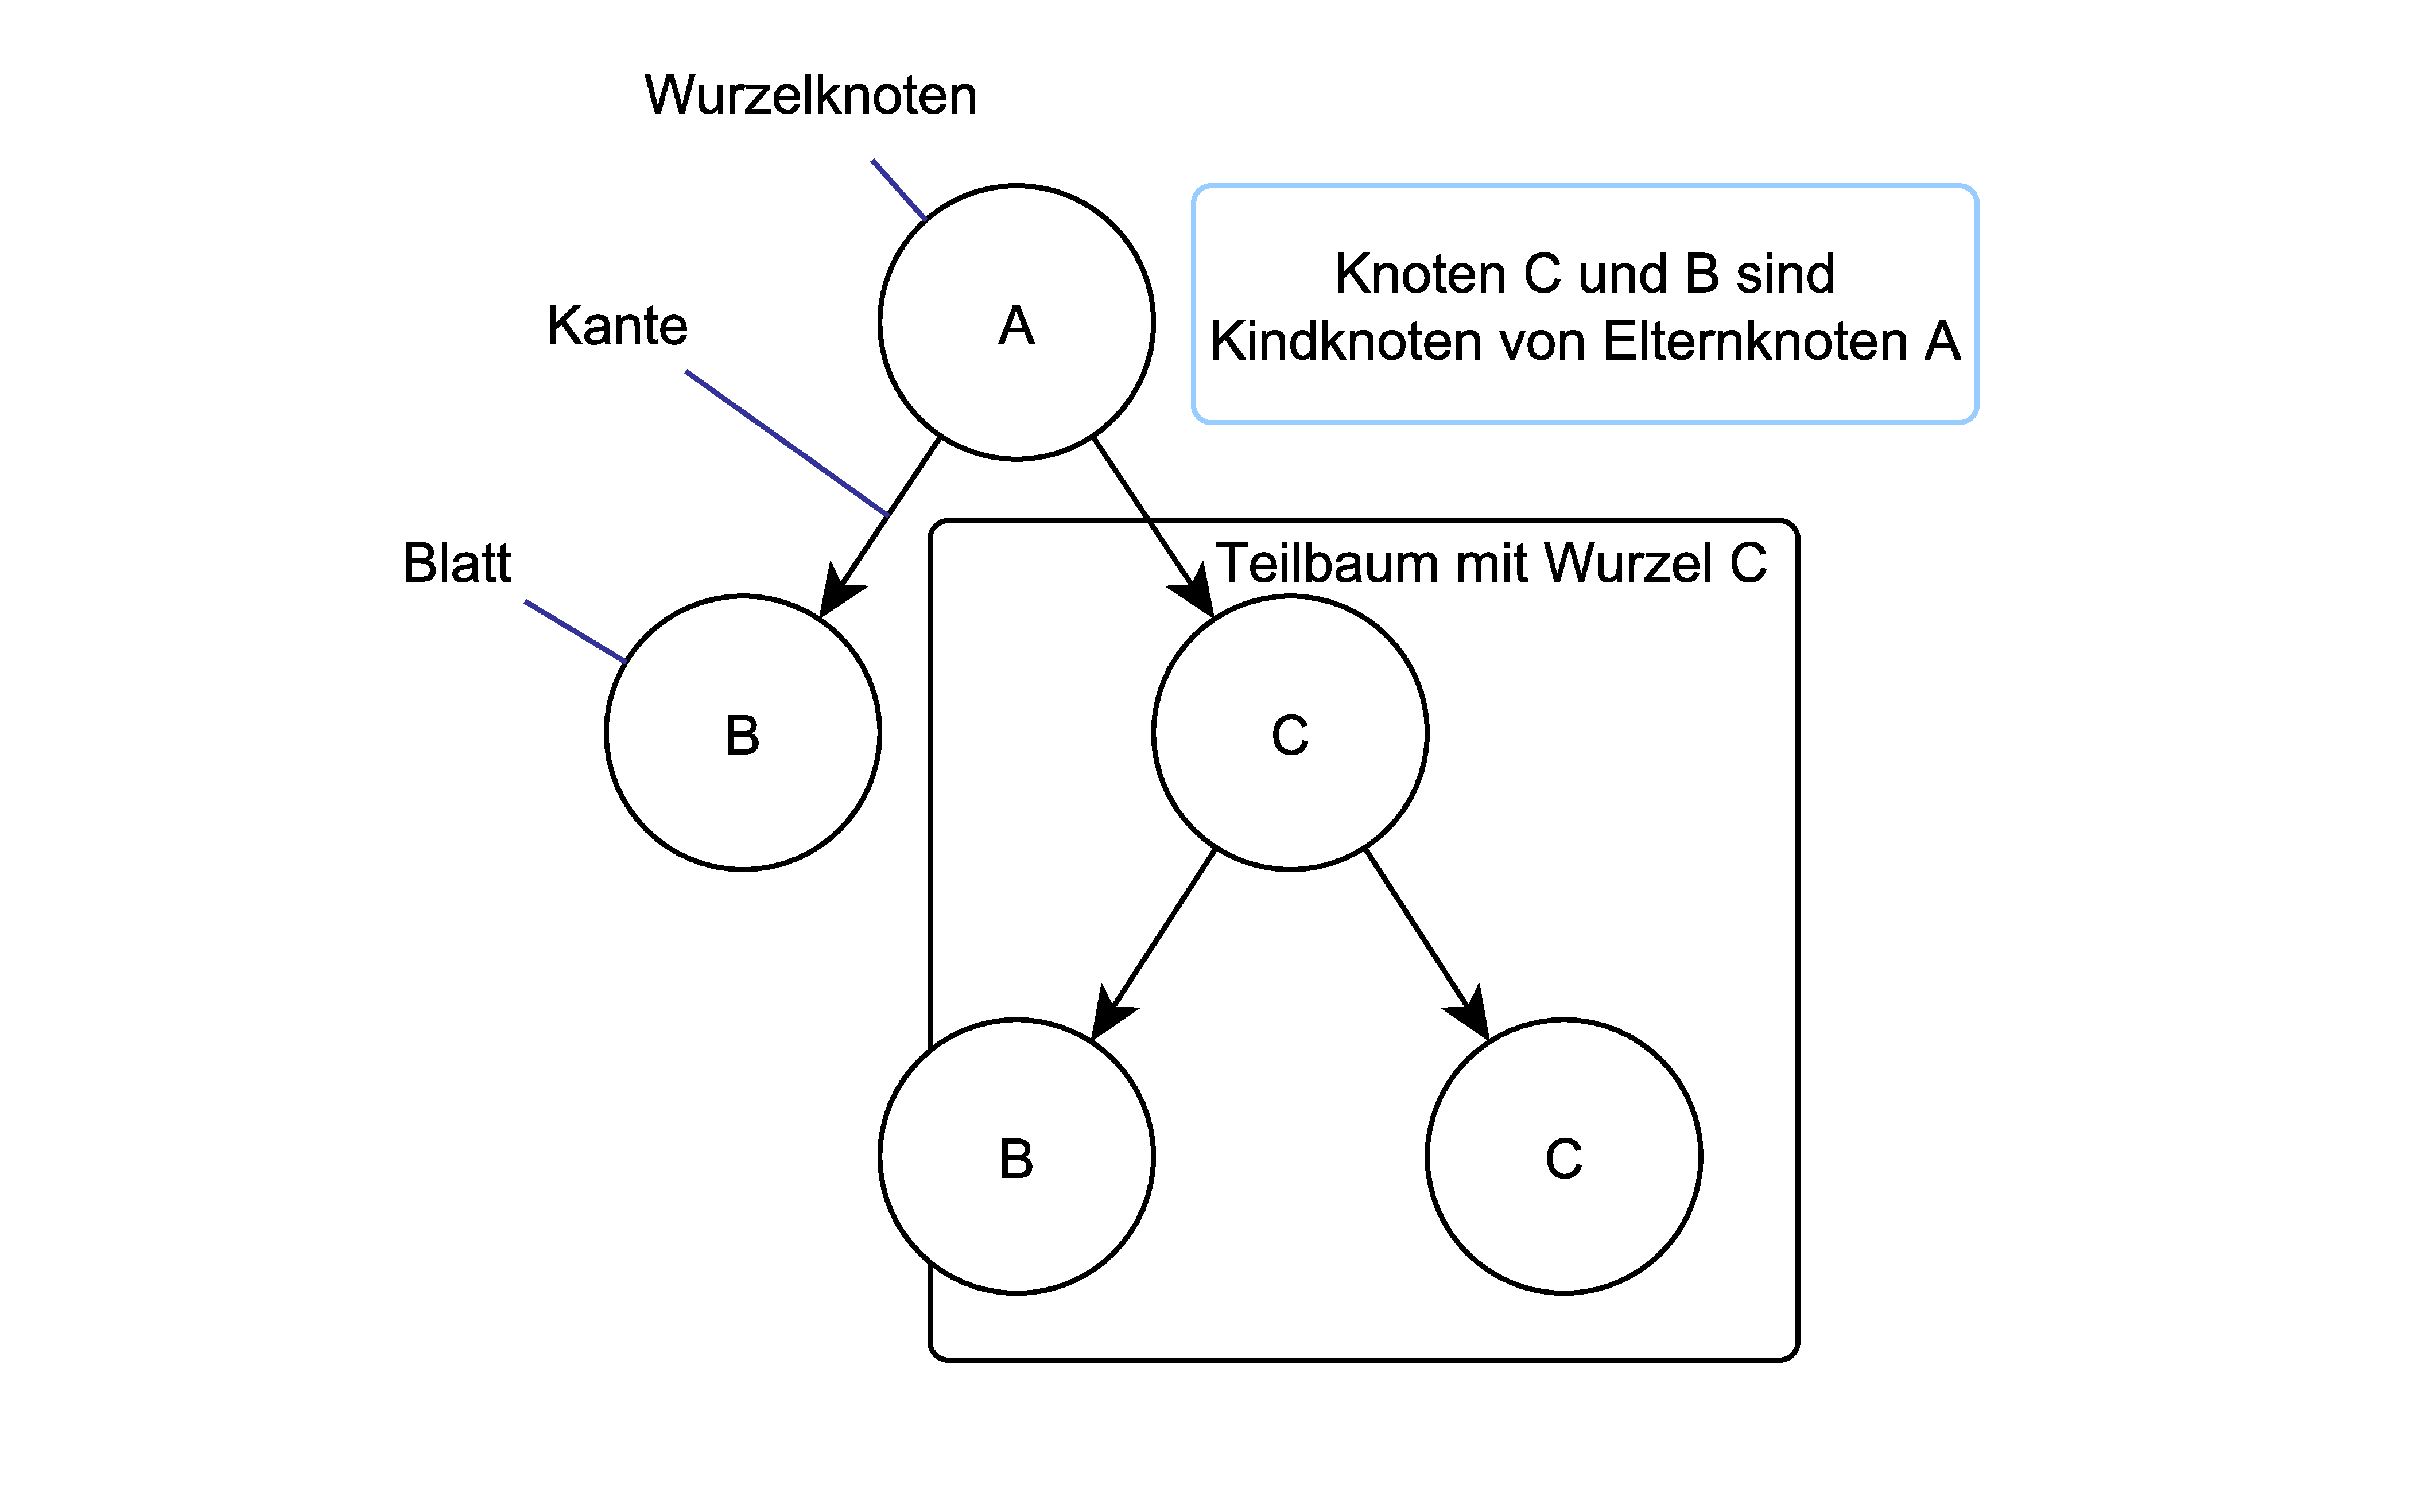
\includegraphics[width=0.7\textwidth]{Suchalgorithmen/suchbaum aufbau.pdf}
	\captionsetup{justification=justified, format=plain}
  \caption{Suchbaum Aufbau}
  \label{fig:suchabaum aufbau}
\end{figure}

\section{Suchalgorithmen}
\label{chap:suchalgorithmen}

Das Suchproblem soll mit seinen Informationen durch einen Suchalgorithmus gel\"{o}st werden. Ein Suchalgorithmus sucht \"{u}ber einen Suchbaum einen Pfad zu dem Ziel. Wie effizient der gefundene Weg, h\"{a}ngt von dem Suchalgorithmus ab. 

Im Bereich der Suchalgorithmen wird zwischen informierten und uniformierten Algorithmen unterschieden. Informierte Algorithmen k\"{o}nnen die Distanz zu dem Ziel mithilfe einer Heuristik sch\"{a}tzen, w\"{a}hrend uniformierte eine solche Sch\"{a}tzung nicht durchf\"{u}hren k\"{o}nnen. Ein weiterer Unterschied ist die Zeit und Speicherkomplexit\"{a}t. W\"{a}hrend uninformierte Algorithmen wie die Tiefensuche weniger Speicher ben\"{o}tigen, k\"{o}nnen sie ineffizient sein, da sie keine Richtung zu dem Ziel ber\"{u}cksichtigen. Informierte Algorithmen sind speicherintensiver, k\"{o}nnen aber Pfade schneller durch die Informationen der Heuristik finden. Unter die uninformierten Suchalgorithmen fallen die Breitensuche, Dijkstra und Tiefensuche. Zu den informierten Suchalgorithmen geh\"{o}rt unter anderem die Bestensuchen.


\subsection{Expansion einer Bestensuche}
\label{chap:bestensuche}

Zu den informierten Suchalgorithmen geh\"{o}rt unter anderem die Bestensuche. Eine Bestensuche arbeitet sich schrittweise \"{u}ber Iterationen mithilfe von Expansionen zu einem Zielknoten vor. Vor der ersten Iteration wird ein Wurzelknoten mit dem Ausgangszustand generiert und der offenen Liste hinzugef\"{u}gt. Die offenen Liste stellt dabei eine Vorrangwarteschlange (Priority Queue) dar. So wird sichergestellt, dass bei der ersten Iteration der Wurzelknoten betrachtet wird.

In der Iteration werden Knoten aus der offenen Liste expandiert. Bei einer Expansion ermittelt der Algorithmus mithilfe der Funktion \textit{TRANSITIONS}$(n)$ alle m\"{o}glichen Kanten \textit{ACTIONS}$(n)$, die vom aktuellen Knoten $n$ ausgehen und zu Kindknoten f\"{u}hren. F\"{u}r die Kindknoten wird eine Bewertung durch die Bewertungsfunktion $f(n)$ berechnet, die je nach Suchalgorithmus variiert. Diese Kindknoten werden daraufhin sortiert nach ihrer Bewertung der offenen Liste hinzugef\"{u}gt. Wenn ein Knoten expandiert wird, wird dieser aus der offenen Liste entfernt. Sollte der gelesene Knoten dem Ziel entsprechen, terminiert der Algorithmus und gibt den Knoten zur\"{u}ck. Ansonsten wird dieser expandiert und die resultierenden Kindknoten der offenen Liste hinzugef\"{u}gt. Die Iteration wird solange fortgef\"{u}hrt bis der Zielknoten gefunden wurde oder sich keine Knoten in der offenen Liste befinden und somit keine Knoten zu dem Ziel f\"{u}hren.

Zu den Bestensuchen geh\"{o}rt unter anderem der Greedy best-first-search und der A*"=Algorithmus, die sich in ihrer Bewertungsfunktion unterscheiden.

Die Abbildung \ref{fig:bestensuche beispiel} veranschaulicht eine abstrakte Suche in einem Suchbaum unter Verwendung der Bestensuche. Dabei sind die gr\"{u}nen Knoten bereits expandierte Knoten, w\"{a}hrend die blauen Knoten zur offenen Liste geh\"{o}ren. Gestrichelte Knoten und Kanten repr\"{a}sentieren nicht entdeckte Elemente, w\"{a}hrend die Bl\"{a}tter des Baums potenzielle Zielknoten darstellen. Der gefundene Pfad [\textit{A, C, E}] weist mit $f(n) = 6$ die geringsten Kosten auf und stellt somit den optimalen Pfad dar.

\lstinputlisting[firstline=0, language=Pseudo, linerange={31-55}, caption={Pseudocode Bestensuche}, label=lst:caption]{code/goap_agent.py}

\begin{figure}[h]
  \centering
  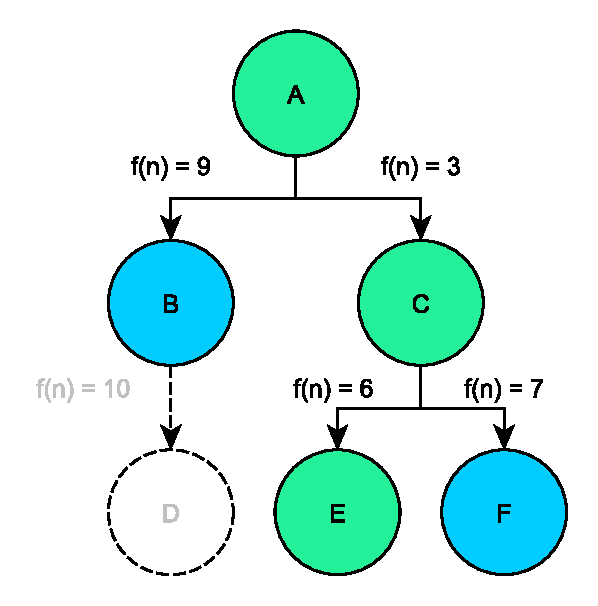
\includegraphics[width=0.7\textwidth]{Suchalgorithmen/bfs suchbaum}
	\captionsetup{justification=justified, format=plain}
  \caption{Suchbeispiel \"{u}ber Bestensuche}
  \label{fig:bestensuche beispiel}
\end{figure}

\subsection{A$^*$ Algorithmus}
\label{chap:a stern suchalgorithmus}

Der A$^*$ Algorithmus geh\"{o}rt zu den informierten und heuristischen Suchverfahren und ist eine Form der Bestensuche. Er ist ein vollst\"{a}ndiger Algorithmus, was bedeutet, dass er einen Pfad zu dem Ziel und findet, wenn einer vorhanden ist. Der A$^$-Algorithmus wird h\"{a}ufig in Routenplanern eingesetzt. Unter anderem benutzten, Game-Engines wie Godot 4.3 den A$^*$-Algorithmus f\"{u}r die Navigation von NPCs.

\subsubsection{Bewertungsfunktion}
\label{chap:a stern bewertungsfunktion}

Bestensuchen benutzen eine Bewertungsfunktion $f(n)$, die dazu dient die Priorit\"{a}t eines Knoten $n$ w\"{a}hrend der Suche zu bewerten. Bei der Bewertungsfunktion des A$^*$ Algorithmus werden dabei alle Pfad-Kosten $g(n)$ vom Ausgangsknoten bis zu dem Knoten $n$ mit der Heuristik $h(n)$ des Knoten $n$ summiert.


\begin{align}
	f(n) = g(n) + h(n)
\end{align}


Mit jeder Erweiterung des Pfades von $n$ zu $n^{\ast}$ steigen die Kosten $g(n)$. Dies liegt an den positiven Aktion-Kosten \textit{ACTIONCOST}$(n,a,n^*)$ der Kanten zwischen den Knoten.


\begin{align}
	g(n) + \textit{ACTIONCOST}(n,a,n^*) + h(n^*) &= g(n^*) + h(n^*)
\end{align}

\subsubsection{Heuristik}

Ein Suchalgorithmus sollte einen Pfad mit m\"{o}glichst geringen Kosten zum Ziel finden, der als optimaler Pfad bezeichnet wird. Ob der A$^*$ Algorithmus einen optimalen Pfad findet, h\"{a}ngt von den Eigenschaften der Heuristik $h(n)$ ab. Eine Heuristik weist die Eigenschaften der Zul\"{a}ssigkeit und Konsistenz auf. Bei einer zul\"{a}ssigen Heuristik werden die Kosten stets untersch\"{a}tzt oder genau gesch\"{a}tzt. Die Kosten einer solchen Heuristik bleiben stets im Intervall $[0, h^{\ast}(n)]$ der tats\"{a}chlichen Kosten des Zielknoten $h^{\ast}(n)$.

\begin{align}
			0 \leq h(n) \leq h^*(n)
\end{align}

Eine konsistente Heuristik, muss gleichzeitig zul\"{a}ssig sein und die Dreiecksungleichung erf\"{u}llen. Umgekehrt muss eine zul\"{a}ssige Heuristik nicht konsistent sein. Die Dreiecksungleichung gibt an, dass die Heuristik $h(n)$ geringer sein soll als die Summe der Aktion $a$ und die Heuristik des folgenden Knoten $h(n^*)$.


\begin{align}
	h(n) \leq \textit{ACTIONCOST}(n,a,n^*) + h(n^*)
\end{align}

Die konsistente Heuristik weist eine st\"{a}rkere Eigenschaft auf, als eine zul\"{a}ssige Heuristik. Der expandierte Knoten bei einer konsistenten Heuristik wird optimal sein, weshalb dieser Knoten nicht erneut in die offene-Liste hinzuf\"{u}gt werden muss.

Bei einer inkonsistenten Heuristik k\"{o}nnen Pfade auftreten, die zu dem selben Zustand f\"{u}hren. Dies f\"{u}hrt dazu, dass mehrere Pfade mit demselben Zustand, aber unterschiedlichen Kosten, in der offenen Liste erscheinen, was zu h\"{o}heren Zeit- und Speicherkosten f\"{u}hrt.

\subsubsection{Beweis f\"{u}r Optimalit\"{a}t}
\label{chap:a stern be}

Arbeitet der A$^*$ Algorithmus mit einer zul\"{a}ssigen oder konsistenten Heuristik, so wird diese den optimalen, kosteng\"{u}nstigsten Pfad zu einem Ziel finden.

Vorraussetzung:
\begin{itemize}
\item Der A$^*$ Algorithmus expandiert auf Knoten mit der geringsten $f(n)$
\item Wir haben zwei m\"{o}gliche Zielknoten:
\begin{itemize}
	\item optimaler Zielknoten: $G_o$
	\item suboptimaler Zielknoten: $G_s_o$
\end{itemize}
\item Eine zul\"{a}ssige Heuristik: $0 \leq h(n) \leq h^*(n)$
\item Einen nicht expandierten Knoten: $n$
\end{itemize}

Beweis:
\begin{enumerate}
	\item Da keine weiteren Schritte vom Zielzustand m\"{o}glich sind gilt: $h(G_o) \land h(G_s_o) = 0$

		\begin{align}
			f(G_o) &= g(G_o) + h(G_o) \\
			f(G_o) &= g(G_o) \\
			f(G_s_o) &= g(G_s_o) + h(G_s_o) \\
			f(G_s_o) &= g(G_s_o)
		\end{align}

	
	Da $G_s_$ suboptimal ist folgt, dass die Pfadkosten $f(n)$ von $G_s_o > G_o$ sind und somit: $f(G_s_o) > f(G_o)$.
	\item Da $g(G_o)$ der tats\"{a}chliche Zielknoten ist und $h^*(n)$ die tats\"{a}chlichen Kosten von $G_o$ sind gilt:
    \begin{align}
			f(n) = g(n) + h(n) &< g(n) + h^*(n) = g(G_o) = f(G_o) \\
			f(n) &< g(G_o)
		\end{align}
\end{enumerate}
Aus 1. und 2. folgt: $f(n) < f(G_o) < f(G_s_o)$. Somit w\"{u}rde der A$^*$ Algorithmus nicht zu $G_s_o$ f\"{u}hren und ist mit einer zul\"{a}ssigen Heuristik optimal.